\section{Question 5}

    To make a task set that is schedulable by EDF but not RM i will find a task set that gives a utilization factor $U = 1$. This will be schedulable with EDF but it is not guaranteed that it is schedulable with RM. To make a task set with $U = 1$ i will use the following equation: $U = \sum_{i=1}^{n} \frac{C_i}{T_i} = 1$. I will use the following task set: 

    \renewcommand{\arraystretch}{1.4}
        \begin{figure}[H]
        \centering
        \begin{minipage}{0.7\textwidth}
            \begin{table}[H]
            \centering
            \begin{tabular}{|l|l|l|}
                \hline
                \textbf{Task}   & \textbf{T=D}  & \textbf{C}  \\ \hline
                A               & 3             & 1           \\ \hline
                B               & 6             & 2           \\ \hline
                C               & 9             & 3           \\ \hline
            \end{tabular}
            \end{table}
        \end{minipage}%
        \caption{Task set}
        \label{fig:Q5tasks}
        \end{figure}
    \renewcommand{\arraystretch}{1.0}

    The task set in figure \ref{fig:Q5tasks} has a utilization factor of $U = \sum_{i=1}^{n} \frac{C_i}{T_i} = \frac{1}{3} + \frac{2}{6} + \frac{3}{9} = 1$. This task set is schedulable with EDF but most likely not with RM. To prove this I will draw the trace for each scheduling algorithm.\\

    \begin{figure}[H]
        \centering
        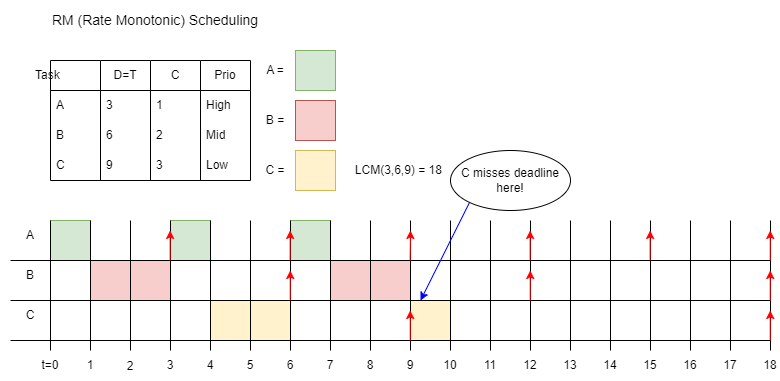
\includegraphics[width=0.8\textwidth]{images/Ass1Q5RM.png}
        \caption{Tracing of the task set with RM scheduling does not work as seen in the figure. The red arrows in the figure indicate the deadlines/period for the tasks.}
        \label{fig:Q5RMtrace}
    \end{figure}

    As seen in figure \ref{fig:Q5RMtrace} the task set is not schedulable with RM scheduling. Task C misses its deadline at $t = 9$.\\

    \begin{figure}[H]
        \centering
        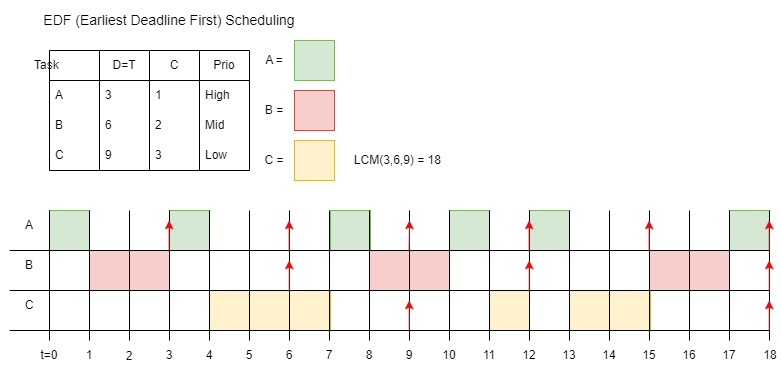
\includegraphics[width=0.8\textwidth]{images/Ass1Q5EDF.drawio.png}
        \caption{Tracing of the task set with EDF scheduling is feasable as seen in the figure. The red arrows in the figure indicate the deadlines/period for the tasks.}
        \label{fig:Q5EDFtrace}
    \end{figure}
        
    As seen in figure \ref{fig:Q5EDFtrace} the task set is schedulable with EDF scheduling. The task set is schedulable with EDF because the task with the earliest deadline is always executed first which guarantees schedulability as long as $U <= 1$.\\